\section{Commercial Instruments} \label{sec:CommercialImpedanceMeasurement}
Most of the major manufacturers of test equipment, such as Keysight Technologies, Rohde \& Schwarz, Tektronix and others produce a range of instruments for characterizing passive components. This section will sample a few of these to research their capabilities, to indicate what a user might want and need. The instruments are chosen based on their perceived price range. 


\subsubsection*{Keysight U1733C}
LCR meters typically come in two different form factors, one is a handheld device, much like a regular multimeter, while the other is a benchtop instrument. The handheld LCR meters, like the Keysight U1733C\cite{KeysightU1733C}, shown in figure \ref{fig:2_2_U1733C}.
\begin{figure}[H]
    \centering
    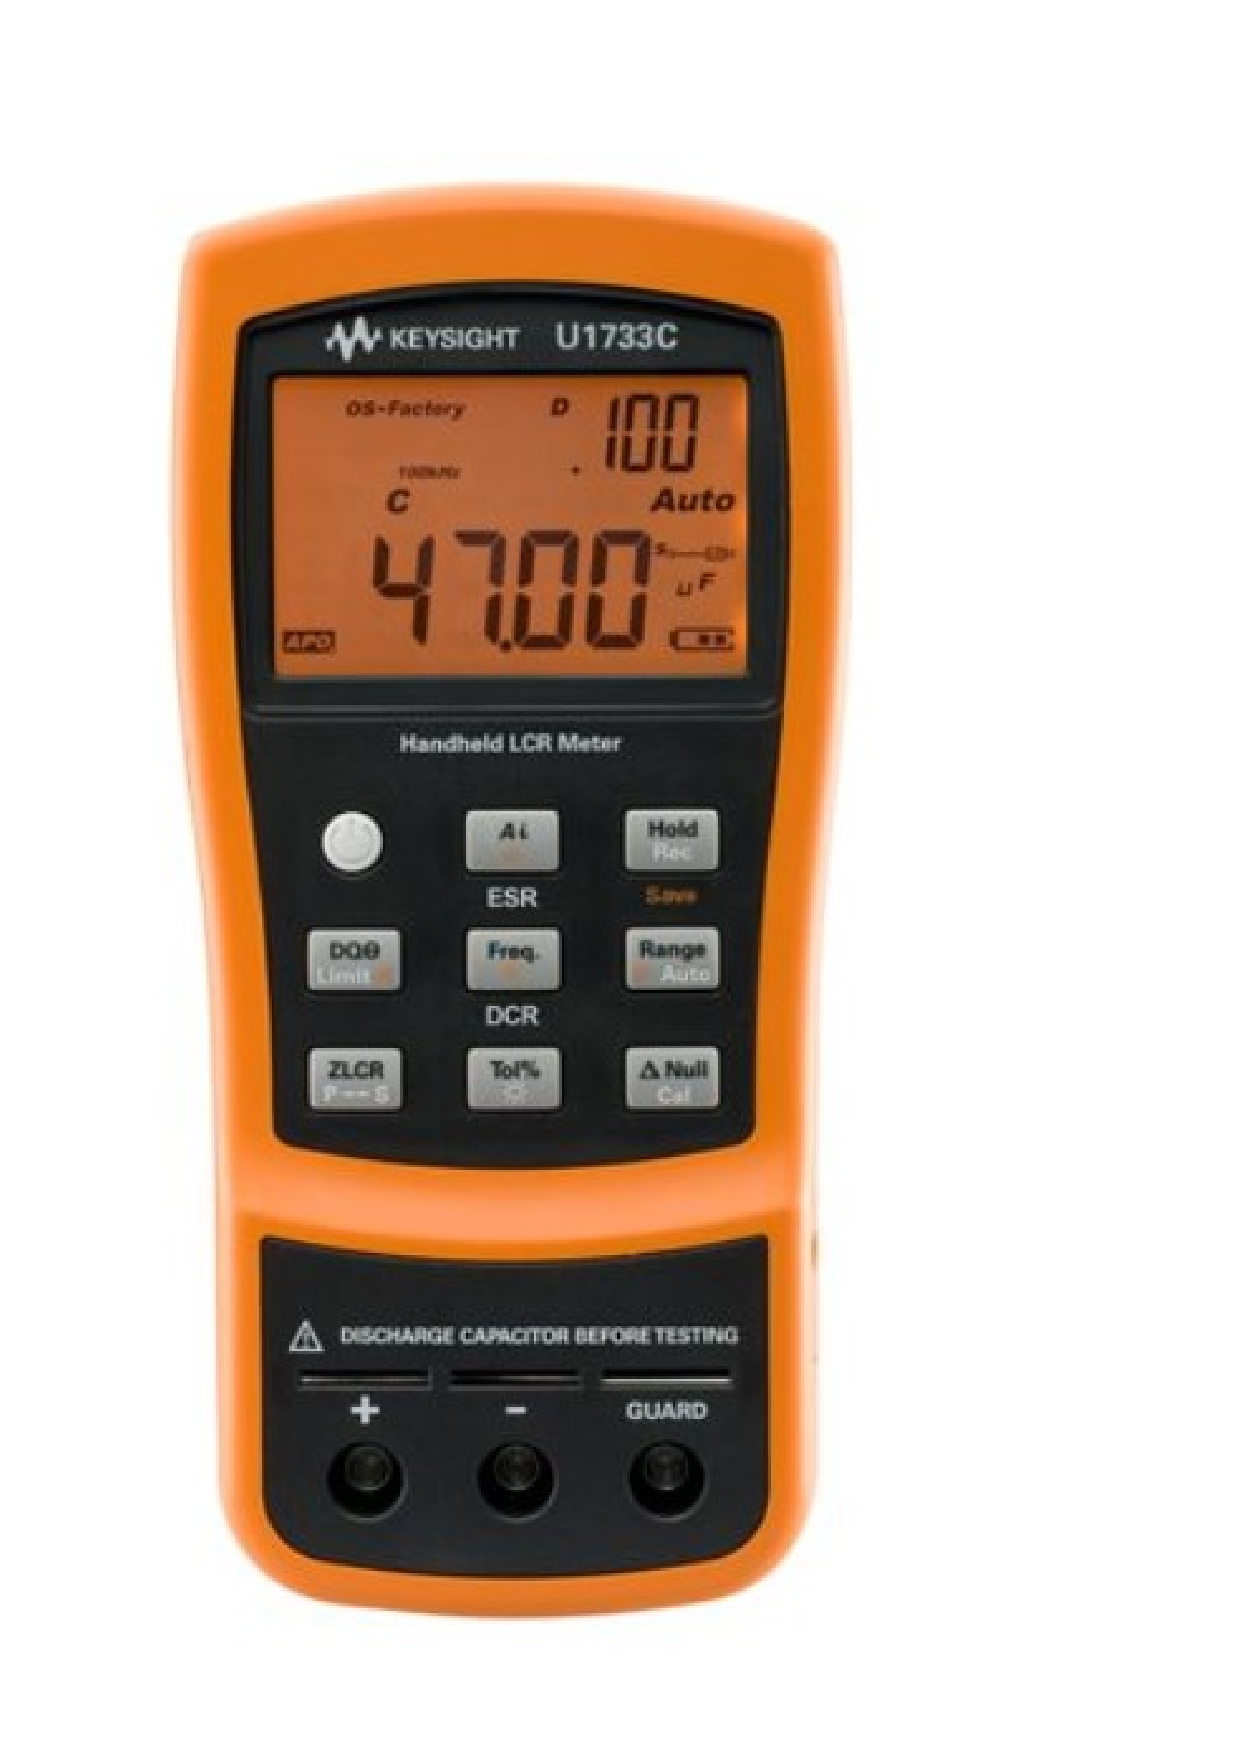
\includegraphics[clip, trim=0 50 0 50, width=0.5\textwidth]{Sections/2_ProblemAnalysis/FIgures/KeysightU1733C.pdf}
    \caption{A handheld Keysight U1733C LCR meter.\cite{KeysightU1733C}}
    \label{fig:2_2_U1733C}
\end{figure}
The U1733C shown on \ref{fig:2_2_U1733C} is meant for, primarily, troubleshooting and repair work and not electronics development purposes, while it is affordable at about 550€, it has limited capabilities. It can measure all the basic parameters such as capacitance, inductance, ESR and display all the derived quantities like dissipation and quality factor, see section \refq{subsec:DerivedQuantities} for further explanation. Numerically, however it can only take these measurements at a pre-determined set of test frequencies in the range \SI[]{100}{\hertz} to \SI[]{100}{\kilo\hertz} with measurement accuracy wearing off in both ends of the impedance range, and at higher frequencies.

Table \refq{tab:2_3_AccuracyTab_U1733C} shows the accuracy of the impedance magnitude for the U1733C at some key impedances at different frequencies. Table \refq{tab:2_3_PhaseAccuracyTab_U1733C} shows the corresponding phase angle accuracy at the same impedances and frequencies. It clearly shows that at the extremes of impedance the accuracy degrades.

\begin{table}[H]
  \begin{tabular}{|m{6.3em}|m{6.3em}|m{6.3em}|m{6.3em}|m{6.3em}|}
  \hline
   Frequency / \nl Applied \nl Impedance & \SIQ{100}{\hertz} & \SIQ{1}{\kilo\hertz} & \SIQ{10}{\kilo\hertz} & \SIQ{100}{\kilo\hertz} \\ \hline
  \SIQ{1}{\ohm}    &   \SIQ{1.2}{\%}   &   \SIQ{1.2}{\%}    &   \SIQ{1.2}{\%}     &   \SIQ{1.5}{\%}      \\ \hline
  \SIQ{10}{\ohm}   &   \SIQ{0.78}{\%}     &  \SIQ{0.78}{\%} & \SIQ{0.78}{\%}  & \SIQ{0.78}{\%}    \\ \hline
  \SIQ{1}{\kilo\ohm}   &   \SIQ{0.23}{\%}     & \SIQ{0.23}{\%}  &  \SIQ{0.23}{\%}  & \SIQ{0.55}{\%} \\ \hline
  \SIQ{100}{\kilo\ohm} &   \SIQ{0.55}{\%}     &  \SIQ{0.55}{\%}  & \SIQ{0.55}{\%}   & \SIQ{0.78}{\%}  \\ \hline
  \SIQ{100}{\mega\ohm} &   \SIQ{6.8}{\%}     &   \SIQ{6.8}{\%}  &  NA   &   NA  \\ \hline
  \end{tabular}
  \caption{Table of selected impedance measurement accuracy of a U1733C. It can be seen that the accuracy degrades at higher frequencies and at the extreme ends of the impedance capabilities.}
  \label{tab:2_3_AccuracyTab_U1733C}
  \end{table}


  \begin{table}[H]
    \begin{tabular}{|m{6.3em}|m{6.3em}|m{6.3em}|m{6.3em}|m{6.3em}|}
    \hline
     Frequency / \nl Applied \nl Impedance & \SIQ{100}{\hertz} & \SIQ{1}{\kilo\hertz} & \SIQ{10}{\kilo\hertz} & \SIQ{100}{\kilo\hertz} \\ \hline
    \SIQ{1}{\ohm}    &   \SIQ{0.69}{\degree} &   \SIQ{0.69}{\degree} &   \SIQ{0.69}{\degree}  &  \SIQ{0.86}{\degree}  \\ \hline
    \SIQ{10}{\ohm}   &   \SIQ{0.45}{\degree}     &  \SIQ{0.45}{\degree} & \SIQ{0.45}{\degree}  & \SIQ{0.45}{\degree}  \\ \hline
    \SIQ{1}{\kilo\ohm}   &  \SIQ{0.13}{\degree}  & \SIQ{0.13}{\degree}  &  \SIQ{0.13}{\degree}  & \SIQ{0.32}{\degree} \\ \hline
    \SIQ{100}{\kilo\ohm} &   \SIQ{0.32}{\degree} &  \SIQ{0.32}{\degree} & \SIQ{0.32}{\degree}  & \SIQ{0.45}{\degree}  \\ \hline
    \SIQ{100}{\mega\ohm} &   \SIQ{3.90}{\degree}     &   \SIQ{3.90}{\degree}  &  NA   &   NA  \\ \hline
    \end{tabular}
    \caption{Table of selected phase angle measurement accuracy of a U1733C. It can be seen that the accuracy degrades at higher frequencies and at the extreme ends of the impedance capabilities.}
    \label{tab:2_3_PhaseAccuracyTab_U1733C}
    \end{table}

\subsubsection*{Rohde \& Schwarz LCX-line}
Rohde \& Schwarz has a benchtop line of LCR meters called the LCX line \cite{RSLCXLCRMeters}. These have tighter specifications for accuracy, a greater range and a more diverse set of displaying the measurements. They also come with a significantly higher price tag, the baseline LCX-200 offering a bandwidth of \SIQ{500}{\kilo\hertz} comes in at 5000 €. This model can then be upgraded through software to the LCX-k201 or LCX-k210, increasing the bandwidth to \SIQ{1}{\mega\hertz} and \SIQ{10}{\mega\hertz}. These software upgrades come at a steep price, with the \SIQ{1}{\mega\hertz} upgrade at 2200 € and the \SIQ{10}{\mega\hertz} upgrade at 8800 € bringing the total price of a \SIQ{1}{\mega\hertz} model to 7200 € and 13800 € for the \SIQ{10}{\mega\hertz} model.

This LCR meter is shown on figure \ref{fig:2_2_RSLCX}. 
\begin{figure}[H]
    \centering
    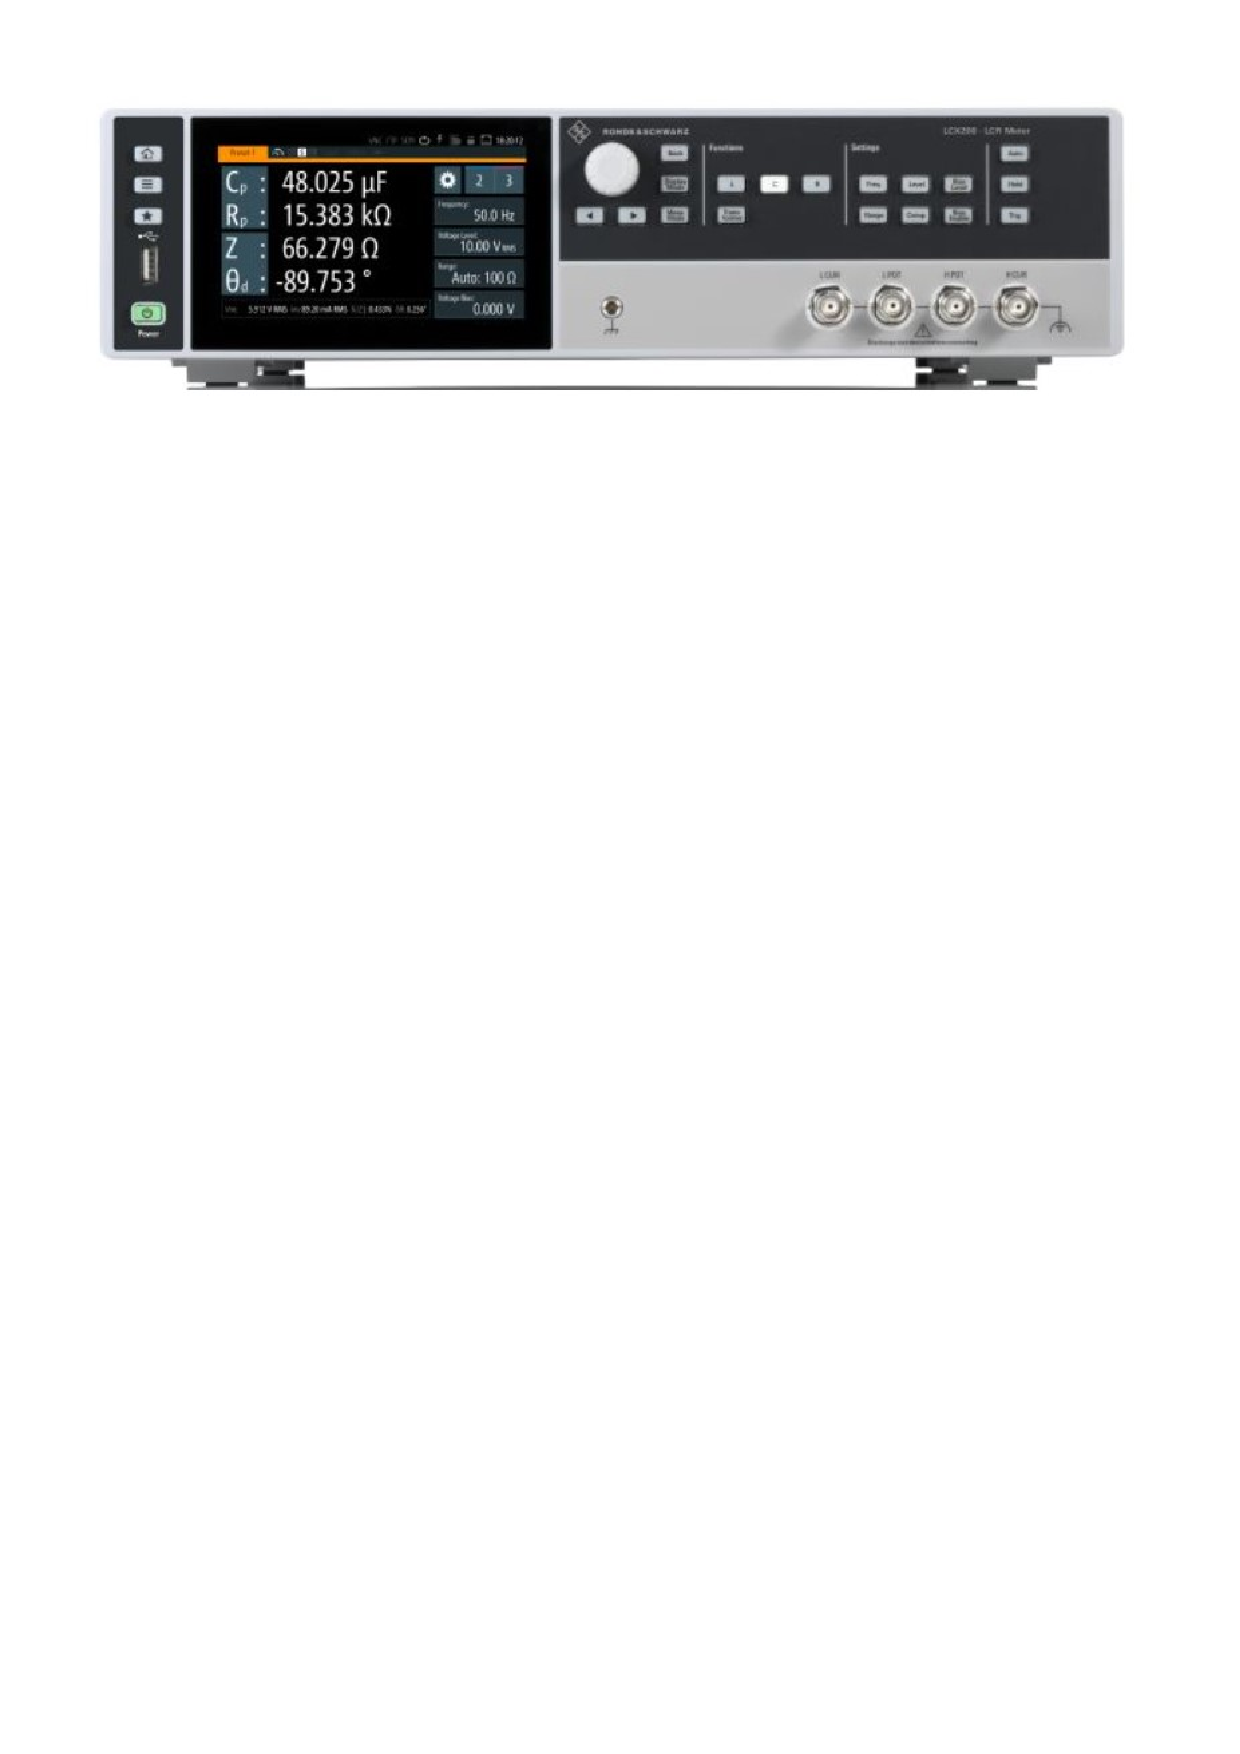
\includegraphics[clip, trim=0 630 0 50, width=1\textwidth]{Sections/2_ProblemAnalysis/FIgures/RSLCXLCR.pdf}
    \caption{A Rohde \& Schwarz LCX LCR meter feature a significantly greater bandwidth when compared to the U1733C, 4-wire kelvin measurements and greater ability to display the measurements.\cite{RSLCXLCRMeters}}
    \label{fig:2_2_RSLCX}
\end{figure}

The Rohde \& Schwarz LCX LCR meter is using kelvin bridge (4-wire) measurements.  This feature is often seen on higher end test equipment in order for the instrument to compensate for the parasitics introduced by the test instruments own test leads. The instrument can be triggered to take measurements externally and be controlled remotely over various network interfaces. The meter also has a sweep function in order to measure the impedance of the DUT over a series of frequency values and can display all the measurements numerically or graphically. Unlike the U1733C this meter is intended for electronic development purposes.

The LCX-line is specified to measure impedances from \SIQ{100}{\milli\ohm} to \SIQ{100}{\mega\ohm}, an extra option can be purchased, allowing it to measure down to \SIQ{10}{\milli\ohm}. The impedance magnitude accuracy of the \SIQ{1}{\mega\hertz} instrument can be seen in table \refq{tab:2_3_AccuracyTab_LCX}, here at some key impedances at different frequencies. The phase angle accuracy can be seen in table \refq{tab:2_3_PhaseAccuracyTab_LCX}. The two tables clearly indicate, that like the U1733C, the higher end LCX meter also has reduced accuracy at the extremes of its impedance ranges, and at higher and lower frequencies.

\begin{table}[H]
  \begin{tabular}{|m{6.3em}|m{6.3em}|m{6.3em}|m{6.3em}|m{6.3em}|}
  \hline
   Frequency / \nl Applied \nl Impedance & \SIQ{10}{\hertz} & \SIQ{1}{\kilo\hertz} & \SIQ{100}{\kilo\hertz} & \SIQ{1}{\mega\hertz} \\ \hline
  \SIQ{1}{\ohm}    &   \SIQ{0.63}{\%}   &   \SIQ{0.63}{\%}    &   \SIQ{0.68}{\%}     &   \SIQ{0.78}{\%}      \\ \hline
  \SIQ{10}{\ohm}   &   \SIQ{0.24}{\%}     &  \SIQ{0.24}{\%} & \SIQ{0.25}{\%}  & \SIQ{0.29}{\%}    \\ \hline
  \SIQ{1}{\kilo\ohm}   &   \SIQ{0.23}{\%}     & \SIQ{0.08}{\%}  &  \SIQ{0.13}{\%}  & \SIQ{0.26}{\%} \\ \hline
  \SIQ{100}{\kilo\ohm} &   \SIQ{0.24}{\%}     &  \SIQ{0.14}{\%}  & \SIQ{0.17}{\%}   & \SIQ{0.34}{\%}  \\ \hline
  \SIQ{100}{\mega\ohm} &   \SIQ{7.05}{\%}     &   \SIQ{7.05}{\%}  &  \SIQ{40.1}{\%}   &   NA  \\ \hline
  \end{tabular}
  \caption{Table of selected impedance measurement accuracy of a R\&S LCX-200 with option K201, increasing the bandwidth to \SIQ{1}{\mega\hertz}. It can be seen that the accuracy degrades at higher frequencies and at the extreme ends of the impedance capabilities.}
  \label{tab:2_3_AccuracyTab_LCX}
  \end{table}

  \begin{table}[H]
    \begin{tabular}{|m{6.3em}|m{6.3em}|m{6.3em}|m{6.3em}|m{6.3em}|}
    \hline
     Frequency / \nl Applied \nl Impedance & \SIQ{100}{\hertz} & \SIQ{1}{\kilo\hertz} & \SIQ{100}{\kilo\hertz} & \SIQ{1}{\mega\hertz} \\ \hline
    \SIQ{1}{\ohm}    &   \SIQ{0.386}{\degree} &   \SIQ{0.386}{\degree} &   \SIQ{0.415}{\degree}  &  \SIQ{0.472}{\degree}  \\ \hline
    \SIQ{10}{\ohm}   &   \SIQ{0.163}{\degree}     &  \SIQ{0.163}{\degree} & \SIQ{0.168}{\degree}  & \SIQ{0.191}{\degree}  \\ \hline
    \SIQ{1}{\kilo\ohm}   &  \SIQ{0.157}{\degree}  & \SIQ{0.071}{\degree}  &  \SIQ{0.099}{\degree}  & \SIQ{0.174}{\degree} \\ \hline
    \SIQ{100}{\kilo\ohm} &   \SIQ{0.163}{\degree} &  \SIQ{0.105}{\degree} & \SIQ{0.122}{\degree}  & \SIQ{0.220}{\degree}  \\ \hline
    \SIQ{100}{\mega\ohm} &   \SIQ{4.064}{\degree}     &   \SIQ{4.064}{\degree}  &  \SIQ{23}{\degree}  &   NA  \\ \hline
    \end{tabular}
    \caption{Table of selected phase angle measurement accuracy of a of a R\&S LCX-200 with option K201, increasing the bandwidth to \SIQ{1}{\mega\hertz}. It can be seen that the accuracy degrades at higher frequencies and at the extreme ends of the impedance capabilities.}
    \label{tab:2_3_PhaseAccuracyTab_LCX}
    \end{table}



\subsubsection*{Wayne-Kerr 6500B}
The Wayne-Kerr 6500B\cite{WayneKerr6500} series is a high-end impedance analyzer for demanding applications. The industry differentiates between \textit{LCR meters} and \textit{Impedance analyzers}. An LCR meter will display it's single point measurements numerically, while an impedance analyzer can do the same but is meant specifically for frequency sweeps and displaying the measurements on graphs. In other words, an impedance analyzer is a more advanced LCR meter. The Wayne-Kerr 6500B is shown on figure \ref{fig:2_2_WayneKerr6500B}. 
\begin{figure}[H]
    \centering
    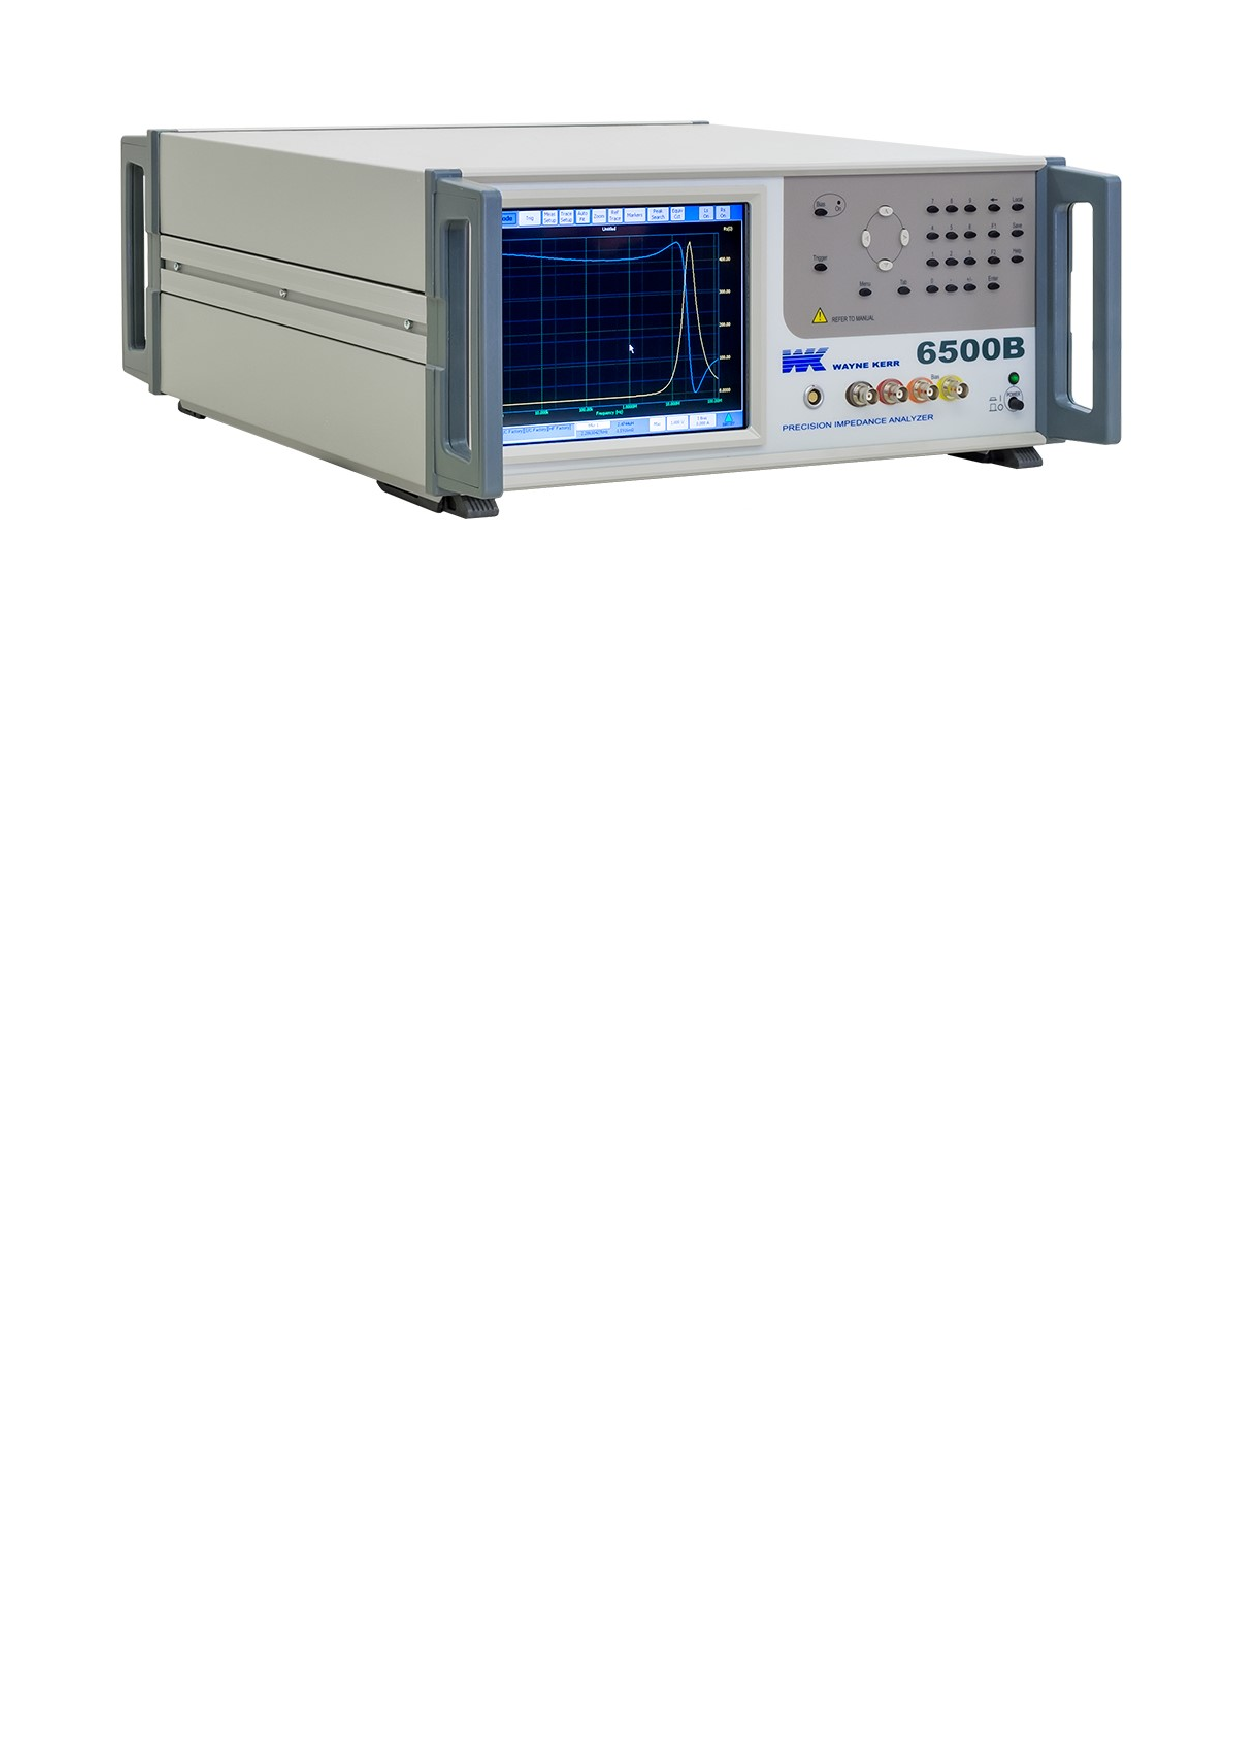
\includegraphics[clip, trim=0 550 0 50, width=1\textwidth]{Sections/2_ProblemAnalysis/FIgures/WayneKerrImpedanceAnalyzer.pdf}
    \caption{A Wayne-Kerr 6500B impedance analyzer. Note how it displays it's measurements graphically.}
    \label{fig:2_2_WayneKerr6500B}
\end{figure}
This impedance analyzer has a test frequency range of \SI[]{20}{\hertz} to \SI[]{120}{\mega\hertz} and has a test frequency resolution of \SI[]{100}{\micro\hertz} and Wayne-Kerr guarantees an accuracy of L, C and R measurements of $\pm 0.05$ \% across the entire frequency range putting this instrument in a different league from the ones previously shown. This impedance analyzer has adjustable DC bias as well, so bias stability can be measured as well. The impedance analyzer can display it's measurements on regular plots but can also show them in polar, or complex, form much like a network analyzer. The price of this instrument is listed as \textit{request quote} putting it far out of reach of even most smaller companies.

\subsubsection*{Summary}
A few LCR meters and impedance analyzers were reviewed, there are many more but it would be impractical to list all of them. It was done in order to analyze what functionality they have. Their functionality and price points are closely related and a table has been made to break down the overall capabilities of each instrument. The results for this can be seen in table \ref{tab:2_3_CapabilityTab}.

\begin{table}[H]
  \begin{tabular}{|m{9.5em}|m{8em}|m{8em}|m{8em}|}
  \hline
    &   Keysight U1733C       & Rohde \& \newline Schwartz \newline LCX-200      & Wayne-Kerr\newline 6500B                 \\ \hline
    Test frequency \nl range$\mathbf{^1}$      &  \SI[]{20}{\hertz} to \SI[]{100}{\kilo\hertz}$\mathbf{^2}$     &    DC-\SI[]{500}{\kilo\hertz},\newline \SI[]{1}{\hertz} steps   & \SI[]{20}{\hertz}-\SI[]{120}{\mega\hertz},\newline  \SI[]{100}{\micro\hertz} steps                                                  \\ \hline
    Accuracy$\mathbf{^3}$            &  [Z]: see table \refq{tab:2_3_AccuracyTab_U1733C}\newline [$\phi$]: see table \refq{tab:2_3_PhaseAccuracyTab_U1733C}     & [Z]: see table \refq{tab:2_3_AccuracyTab_LCX}\newline [$\phi$]: see table \refq{tab:2_3_PhaseAccuracyTab_LCX}       &[Z] $\pm 0.05$\%\newline [$\phi$] $\pm 0.0005$\degree                                                    \\ \hline
    Interface Type            &  Simple$\mathbf{^4}$\nl LCD, buttons    & Touchscreen & Touchscreen \\ \hline
    Measurement mode          &   2-wire    & 4-wire      & 4-wire                                  \\ \hline
    Auto ranging              &   Yes    & Yes      & Yes                                           \\ \hline
    Adj. DC Bias range        &   No    & \SIQ{40}{\volt}DC$\mathbf{^5}$      & $\pm$\SIQ{40}{\volt}DC           \\ \hline
    Frequency sweep           &   No    & Yes$\mathbf{^6}$      & Yes                               \\ \hline
    Data logging              &   No    & Yes      & Yes                                            \\ \hline
    Component binning         &   No    & Yes      & Yes                                            \\ \hline
    Graph data point          &   No    & Yes      & Yes                                            \\ \hline
    Complex plane plots       &   No    & No       & Yes                                             \\ \hline
    Network access            &   No    & Yes      & Yes                                  \\ \hline
    Price point               & <1000€   & 5000€ $\mathbf{^7}$   & Undisclosed                                    \\ \hline
  \end{tabular}
  \caption*{
    \raggedright
    $\mathbf{^1}$ The frequency range depends on the model.\\
    $\mathbf{^2}$ The test frequencies for the U1733C are in pre-determined steps.\\
    $\mathbf{^3}$ \textit{Z} refers to impedance measurement accuracy. \textit{$\phi$} refers specifically to the phase measurement.\\
    $\mathbf{^4}$ \textit{simple} refers to the instruments U/I being a few buttons and an LCD display as shown on figure \ref{fig:2_2_U1733C}.\\
    $\mathbf{^5}$ The Rohde \& Schwartz LCX DC bias setting is an extra software options that can be purchased\\
    $\mathbf{^6}$ The Rohde \& Schwartz LCX can do frequency sweeps if an extra software option is purchased.\\
    $\mathbf{^7}$ The price of a \SIQ{500}{\kilo\hertz} LCX-200 version without any options. \\
  }
  \caption{A summary of the capabilties of the 3 instruments.}
  \label{tab:2_3_CapabilityTab}
\end{table}

As shown in table \ref{tab:2_3_CapabilityTab} there is a clear distinction in the level of features available at different price points and the major differentiator in their price is the instruments accuracy and test frequency range. The U1733C is affordable for most individuals but lacks a lot of the functions and range available at higher price brackets. The LCX and 6500B will have significantly more advanced hardware and a major difference between these two is there test frequency ranges. It is noteworthy how some of their features are due to them having more advanced software and interfaces. Some of these features could be made available in a lower price bracket with software alone. 


